\documentclass[12pt, a4paper]{report}

\usepackage[utf8x]{inputenc}
\usepackage{amsmath}
\usepackage[english,russian]{babel}
\usepackage{cmap}
\usepackage{listings}
\usepackage{geometry}
 \geometry{
 a4paper,
 total={170mm,257mm},
 left=20mm,
 top=20mm,
 }

\usepackage{graphicx}
\graphicspath{ {../images/.} }

\begin{document}
\section*{Введение}
\textbf{Устойчивость} - свойство САР(системы автоматического регулирования) возвращаться к устойчивому установившемуся режиму после оказания внешнего воздействия. \\

Устойчивость САР оценивается по:
\begin{enumerate}
  \item Статические характеристики САР
  \item По экспериментально полученным переходным процессам
  \item По математическому описанию САР
\end{enumerate}

\textbf{Условие устойчивости по математическому описанию САР}
\[ \lim\limits_{ t\rightarrow\infty}{\varphi_{пер}(t)} = 0\]
\[ \lim\limits_{ t\rightarrow\infty}{\omega(t)} = 0\]
\[ \varphi_{пер}(t) = C * e^{pt}, \]
\centerline{где p - корни характеристического уравнения}
\begin{displaymath}
A_{3}\frac{d^{3}\varphi}{dt^{3}} + A_{2}\frac{d^{2}\varphi}{dt^{2}} + A_{1}\frac{d\varphi}{dt} + A_{0}\varphi = 0
\end{displaymath}

Оценка устойчивости МАР по расположению корней характеристического уравнения.
Для устойчивости САР необходимо и достаточно, чтобы все корни лежила в левой полуплоскости плоскости корней \\

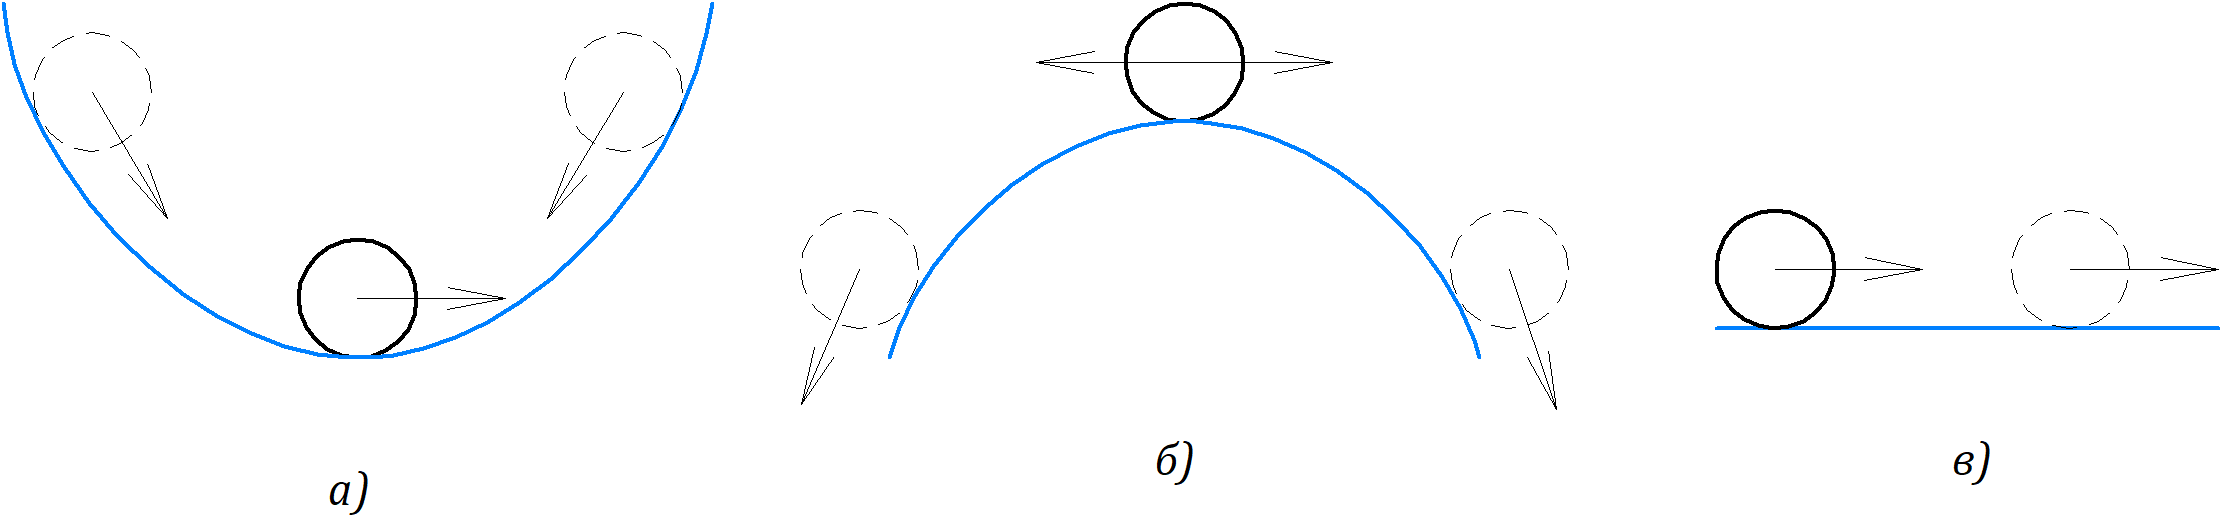
\includegraphics[width=15cm, height=4cm]{condition}


\textbf{Условие выполняется если корни отрицательны или комплексно сопряженные с отрицательной везественной частью}
\begin{displaymath}
\varphi_{\text{пер}}(t) = C_{1}e^{p_{1}t} + C_{2}e^{p_{2}t} + C_{3}e^{p_{3}t} =
\frac{C_{1}}{e^{t}} + \frac{C_{2}}{e^{2t}} + \frac{C_{3}}{e^{3t}}
\end{displaymath}

Для систем высоких порядков нахождение корней становится трудоемким и желательно знать признаки устойчивости
САР без нахождения корней характеристического уравнения

\end{document}